Poderíamos definir outros pontos críticos no modelo de percolação. Por exemplo,  
lembrando que $\xip$ é o valor esperado do volume do aglomerado aberto da origem, 
seja 
\beq 
\pt=\sup\{p:\xip<\infty\}. 
\eeq 
A prova da Proposição~\ref{prop:trans1} mostra que $\pt$ está bem definido e é
positivo.
É claro que $\pt\leq p_c$ (pois se $\tep=\p(|C|=\infty)>0)$ então $\xip=\infty$). 
 
Neste capítulo,  veremos que $\pt=\pce$, eliminando a existência de uma fase 
intermediária $(\pt,\pce)$ e estabelecendo a assim chamada {\em unicidade} do ponto 
crítico. 
 
Este resultado foi provado independentemente por Menshikov \cite{kn:M} e  
Aizenman e Barsky \cite{kn:AB} por argumentos diferentes (para $d$ geral; em 2 dimensões foi provado 
por Kesten \cite{kn:K1} como conseqüência de que, neste caso, $\pce=1/2$). Mostraremos a seguir o 
argumento de Menshikov (com uma melhoria de Kesten, não publicada). 
 
Sejam $\sn$ a esfera $L_1$  em $\zd$ de raio $n$ com centro na origem, isto é 
$$\sn=\{x\in\zd:||x||_1\leq n\}$$ e  $A_n$ o evento de que existe um caminho 
aberto da origem à fronteira de $\sn$. 

\vs

\bte[Menshikov]
\label{teo:teo1} 
Se $p<\pce$, então para algum $\psp>0$ 
\beq 
\label{eq:exp0}
\p(A_n)\leq e^{-\psp n}\quad\mbox{para todo $n$.} 
\eeq  
\ete 

%\nopagebreak
 
\vs

\bco
\label{cor:exp}
$\xip<\infty$ se $p<\pce$.
\eco

\vs

\bob
Na fase supercrítica $\xip=\infty$, obviamente.
Prova-se tam\-bém \cite{kn:G} que $$\lim_{p\ua\pce}\xip=\infty.$$
\eob

\vs

\noindent {\bf Prova do Corolário~\ref{cor:exp}.}

O Teorema~\ref{teo:teo1} estabelece o decaimento exponencial da distribuição
do raio de $C$.
De~(\ref{eq:exp0}) concluimos que 
\beq
\label{eq:exp1}
\p(|C|\geq n)\leq e^{-\psp' n^{1/d}},
\eeq
com $\psp'>0$. Logo,
$$\xip=\sum_{n\geq1}\p(|C|\geq n)<\infty. \bo$$

\vs

\bob
\label{ob:exp1}
(\ref{eq:exp1}) estabelece decaimento subexponencial da distribuição de 
$|C|$. Com um pouco mais de trabalho, mostra-se o decaimento exponencial desta
distribuição (vide~\cite{kn:G}).
\eob

\vs

A prova do Teorema~\ref{teo:teo1} será  apresentada em uma introdução mais 
três partes. 
 
\vspace{.5cm} 
 
\noindent {\bf Introdução} 
 
Defina 
\beq 
\gpn=\p(A_n). 
\eeq 
 
Note que $\gpn\da\tep$ quando $n\ua\infty$. Logo, se $p<\pce$, existe $p'$ satisfazendo 
$p<p'<\pce$ e portanto $$\lim_{n\to\infty}g_{p'}(n)=\theta(p')=0.$$ 
O problema é mostrar que para algum $p'$, se  
$\lim_{n\to\infty}g_{p'}(n)=0$ então para $p<p'$ 
$$\gpn\leq e^{-\psp n}.$$ 
Queremos limitar $\gpn$ superiormente em termos de $g_{p'}(n)$ e mais alguma coisa 
(é preciso melhorar a cota trivial $\gpn\leq g_{p'}(n)$). 
 
\vspace{.5cm} 
 
\noindent {\bf Parte 1} 
 
Como já vimos no Capítulo 2, Seção 3, a fórmula de Russo produz a  
seguinte desigualdade para $0<\a\leq\b\leq1$. 
\beq 
\gan\leq\gbn\exp\left(-\int_{\a}^{\b}\ep(N(A_n)|A_n)dp\right), 
\eeq 
onde $N(A_n)$ é o número de elos pivotais para o evento $A_n$. 
 
\vspace{.5cm} 
 
\noindent {\bf Parte 2} 
 
Para um dado $\b$, seja $M$ o raio (aleatório) do aglomerado aberto da 
origem (isto é, $\max_{x\in C}||x||_1$ ou, equivalentemente,  
$\max\{k:A_k$ ocorre\}). Note que se $\tep>0$, então $M=\infty$ com 
probabilidade positiva e se $\tep=0$ então $M$ é uma variável aleatória 
finita com valores inteiros.  
 
Sejam $M_1,M_2,\ldots$ variáveis aleatórias independentes 
com a mesma distribuição de $M$. Mostraremos mais adiante  
que  
\beq 
\p(N(A_n)\geq k|A_n)\geq P((1+M_1)+\ldots+(1+M_k)\leq n), 
\eeq 
para todo $k\geq0$, o que relaciona $N(A_n)$ (condicionado a  
$A_n$) a um processo de 
renovação. Usando métodos usuais em tais processos, conclui-se que 
\beqn
\nonumber
\ep(N(A_n)|A_n)\=\sum_{k=1}^\infty\p(N(A_n)\geq k|A_n)\\ 
\nonumber
\ge \sum_{k=1}^\infty P((1+M_1)+\ldots+(1+M_k)\leq n)\\ 
\label{eq:wald}
\ge \frac{n}{E(1+M\wedge n)}-1=\frac{n}{\sum_{i=0}^n\gpi}-1. 
\eeqn 

 
\vspace{.5cm} 
 
\noindent {\bf Parte 3} 
 
Combinam-se as partes 1 e 2 para obter para $0<\a\leq\b\leq1$: 
 
\beq 
\label{eq:eq3} 
\gan\leq\gbn\exp\left[(\b-\a)-(\b-\a)\frac{n}{\sum_{i=0}^n g_\beta(i)}\right]. 
\eeq 
 
Da desigualdade acima, concluiremos que  
\beq 
\label{eq:eq4} 
\sum_{i=0}^\infty g_\beta(i)<\infty, 
\eeq 
do que segue o teorema. 
 
\vspace{.5cm} 
 
Em seguida apresentaremos as partes 2 e 3 em detalhes. 
 
\vspace{.5cm} 
 
\noindent {\bf Parte 2} 
 
Sejam $\{e_1,e_2,\ldots,e_m\}$ os elos pivotais abertos para $A_n$ na ordem 
com que são atingidos por um caminho aberto da origem  
até $\del S_n$. (Note que a ordem é a mesma para qualquer tal caminho devido 
à pivotalidade.) Escreva $e_j$ como $(x_j,y_j)$ (Na "ordem correta". 
Veja a Figura~\ref{fig:exp1}.). 

\bef
%\font\thinlinefont=cmr5
\mbox{\beginpicture
\setcoordinatesystem units < 0.800cm, 0.800cm>
\unitlength= 0.800cm
\linethickness=1pt
\setplotsymbol ({\makebox(0,0)[l]{\tencirc\symbol{'160}}})
\setshadesymbol ({\thinlinefont .})
\setlinear
%
% Fig POLYLINE object
%
\linethickness= 0.500pt
\setplotsymbol ({\thinlinefont .})
\plot  3.778 16.542  3.778 16.542 /
%
% Fig POLYLINE object
%
\linethickness= 0.500pt
\setplotsymbol ({\thinlinefont .})
\putrule from  3.778 16.542 to  3.778 16.542
%
% Fig POLYLINE object
%
\linethickness=1pt
\setplotsymbol ({\makebox(0,0)[l]{\tencirc\symbol{'160}}})
\plot  7.588 16.542 12.033 20.987 /
%
% Fig POLYLINE object
%
\linethickness=1pt
\setplotsymbol ({\makebox(0,0)[l]{\tencirc\symbol{'160}}})
\plot 12.033 20.987 16.478 16.542 /
%
% Fig POLYLINE object
%
\linethickness= 0.500pt
\setplotsymbol ({\thinlinefont .})
%
% arrow head
%
\plot 12.097 21.368 12.033 21.622 11.970 21.368 /
%
\putrule from 12.033 21.622 to 12.033 11.462
%
% Fig POLYLINE object
%
\linethickness=1pt
\setplotsymbol ({\makebox(0,0)[l]{\tencirc\symbol{'160}}})
\plot  7.588 16.542 12.033 12.097 /
%
% Fig POLYLINE object
%
\linethickness=1pt
\setplotsymbol ({\makebox(0,0)[l]{\tencirc\symbol{'160}}})
\plot 16.478 16.542 12.033 12.097 /
%
% Fig POLYLINE object
%
\linethickness=1pt
\setplotsymbol ({\makebox(0,0)[l]{\tencirc\symbol{'160}}})
\putrule from 12.668 18.447 to 10.741 18.447
\putrule from 10.763 18.447 to 10.763 17.790
\putrule from 10.763 17.812 to 12.668 17.812
%
% Fig POLYLINE object
%
\linethickness=1pt
\setplotsymbol ({\makebox(0,0)[l]{\tencirc\symbol{'160}}})
\putrule from 10.763 17.812 to 10.763 15.272
%
% Fig POLYLINE object
%
\linethickness=1pt
\setplotsymbol ({\makebox(0,0)[l]{\tencirc\symbol{'160}}})
\putrule from 10.763 16.542 to  9.471 16.542
\putrule from  9.493 16.542 to  9.493 15.250
\putrule from  9.493 15.272 to 14.573 15.272
%
% Fig POLYLINE object
%
\linethickness=1pt
\setplotsymbol ({\makebox(0,0)[l]{\tencirc\symbol{'160}}})
\putrule from 11.398 15.272 to 11.398 12.732
%
% Fig POLYLINE object
%
\linethickness=0pt
\setplotsymbol ({\thinlinefont \ })
\putrule from 13.303  9.557 to 14.573  9.557
%
% Fig POLYLINE object
%
\linethickness=0pt
\setplotsymbol ({\thinlinefont \ })
\putrule from 13.303  9.557 to 14.573  9.557
%
% Fig POLYLINE object
%
\linethickness=0pt
\setplotsymbol ({\thinlinefont \ })
\putrule from 19.018 15.907 to 19.018 11.462
%
% Fig POLYLINE object
%
\linethickness=0pt
\setplotsymbol ({\thinlinefont \ })
\putrule from  8.223  9.557 to 10.763  9.557
%
% Fig POLYLINE object
%
\linethickness=1pt
\setplotsymbol ({\makebox(0,0)[l]{\tencirc\symbol{'160}}})
\putrule from 12.668 18.447 to 12.668 16.542
%
% Fig POLYLINE object
%
\linethickness=1pt
\setplotsymbol ({\makebox(0,0)[l]{\tencirc\symbol{'160}}})
\putrule from 12.668 17.177 to 12.011 17.177
\putrule from 12.033 17.177 to 12.033 16.520
\putrule from 12.033 16.542 to 12.668 16.542
%
% Fig POLYLINE object
%
\linethickness=1pt
\setplotsymbol ({\makebox(0,0)[l]{\tencirc\symbol{'160}}})
\putrule from 14.573 15.272 to 14.573 14.637
%
% Fig POLYLINE object
%
\linethickness=1pt
\setplotsymbol ({\makebox(0,0)[l]{\tencirc\symbol{'160}}})
\plot 10.763 17.177 10.763 17.177 /
%
% Fig POLYLINE object
%
\linethickness= 0.500pt
\setplotsymbol ({\thinlinefont .})
\plot 10.763 17.177 10.763 17.177 /
%
% Fig POLYLINE object
%
\linethickness= 0.500pt
\setplotsymbol ({\thinlinefont .})
\putrule from  6.953 16.542 to  9.493 16.542
%
% Fig POLYLINE object
%
\linethickness= 0.500pt
\setplotsymbol ({\thinlinefont .})
\putrule from 11.398 16.542 to 17.113 16.542
%
% arrow head
%
\plot 16.859 16.478 17.113 16.542 16.859 16.605 /
%
%
% Fig POLYLINE object
%
\linethickness= 0.500pt
\setplotsymbol ({\thinlinefont .})
\setdashes < 0.1270cm>
\plot 10.763 17.177 10.922 17.177 /
%
% Fig POLYLINE object
%
\linethickness= 0.500pt
\setplotsymbol ({\thinlinefont .})
\setsolid
\putrule from 10.763 16.542 to 11.557 16.542
%
% Fig POLYLINE object
%
\linethickness=1pt
\setplotsymbol ({\makebox(0,0)[l]{\tencirc\symbol{'160}}})
\putrule from 14.573 15.907 to 14.573 15.272
%
% Fig POLYLINE object
%
\linethickness=1pt
\setplotsymbol ({\makebox(0,0)[l]{\tencirc\symbol{'160}}})
\putrule from 13.938 15.907 to 13.938 13.980
\putrule from 13.938 14.002 to 12.668 14.002
%
% Fig POLYLINE object
%
\linethickness=1pt
\setplotsymbol ({\makebox(0,0)[l]{\tencirc\symbol{'160}}})
\putrule from 12.668 12.732 to 12.668 14.659
\putrule from 12.668 14.637 to 10.741 14.637
\putrule from 10.763 14.637 to 10.763 13.980
\putrule from 10.763 14.002 to 12.033 14.002
%
% Fig POLYLINE object
%
\linethickness=1pt
\setplotsymbol ({\makebox(0,0)[l]{\tencirc\symbol{'160}}})
\putrule from 10.128 17.177 to 10.128 15.885
\putrule from 10.128 15.907 to  8.858 15.907
%
% Fig POLYLINE object
%
\linethickness=1pt
\setplotsymbol ({\makebox(0,0)[l]{\tencirc\symbol{'160}}})
\putrule from 11.398 19.082 to 11.398 17.812
%
% Fig POLYLINE object
%
\linethickness=1pt
\setplotsymbol ({\makebox(0,0)[l]{\tencirc\symbol{'160}}})
\putrule from 12.668 19.082 to 12.668 18.447
%
% Fig POLYLINE object
%
\linethickness=1pt
\setplotsymbol ({\makebox(0,0)[l]{\tencirc\symbol{'160}}})
\putrule from 12.668 16.542 to 12.668 15.907
%
% Fig POLYLINE object
%
\linethickness=1pt
\setplotsymbol ({\makebox(0,0)[l]{\tencirc\symbol{'160}}})
\putrule from 12.668 16.542 to 13.303 16.542
%
% Fig POLYLINE object
%
\linethickness=1pt
\setplotsymbol ({\makebox(0,0)[l]{\tencirc\symbol{'160}}})
\putrule from 12.668 17.177 to 13.144 17.177
%
% Fig POLYLINE object
%
\linethickness=1pt
\setplotsymbol ({\makebox(0,0)[l]{\tencirc\symbol{'160}}})
\putrule from 13.144 17.177 to 13.303 17.177
%
% Fig TEXT object
%
\put {$0$} [lB] at 11.716 16.066
%
% Fig TEXT object
%
\put {$e_1$} [lB] at 12.827 17.335
%
% Fig TEXT object
%
\put {$e_2$} [lB] at 10.922 17.335
%
% Fig TEXT object
%
\put {$e_3$} [lB] at 10.922 16.701
%
% Fig TEXT object
%
\put {$e_4$} [lB] at 10.922 15.431
\linethickness=0pt
\putrectangle corners at  3.778 21.622 and 19.018  9.557
\endpicture}

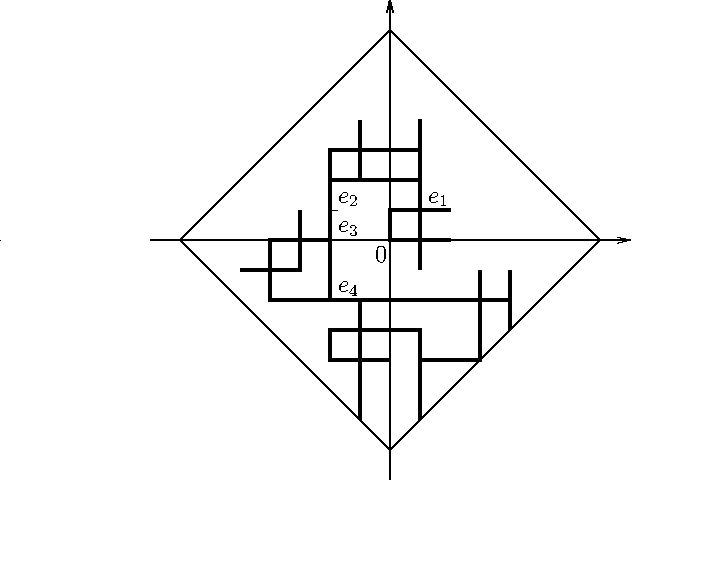
\includegraphics{piv1}
\caption{Figura do aglomerado da origem em $S_7$. Há exatamente 4 elos
pivotais para $A_7$ nesta configuração, denotados $e_1$, $e_2$, $e_3$ e $e_4$.}
\label{fig:exp1}
\eef

Os elos do aglomerado da origem entre os elos pivotais sucessivos formam
{\em salsichas}. O aglomerado da origem em $\sn$ pode ser visto então como
como salsichas de elos conectadas por elos pivotais.
 
Sejam  
\beqnn 
\ro_1\=||x_1||_1\\ 
\ro_2\=||y_1-x_2||_1\\ 
&\vdots&\\ 
\ro_m\=||y_{m-1}-x_m||_1,  
\eeqnn          
e $\rho_i=\infty$ para $i>m$.
$\rho_1,\ldots,\rho_m$ representam os {\em raios} das salsichas sucessivas.

Então $N(A_n)\geq k$ se  
$$(\ro_1+1)+(\ro_2+1)+\ldots+(\ro_k+1)\leq n,$$ ou seja, 
$$\ro_1+\ldots+\ro_k\leq n-k.$$ 
Logo, 
\beq 
\label{eq:conf}
\p(N(A_n)\geq k|A_n)\geq\p(\ro_1+\ldots+\ro_k\leq n-k|A_n). 
\eeq 

Queremos mostrar que 
\beq 
\label{eq:eq2} 
\p(\ro_1+\ldots+\ro_k\leq n-k|A_n)\geq\p(M_1+\ldots+M_k\leq n-k), 
\eeq para todo $n$ e $k$, 
onde $M_1,M_2,\ldots$ são variáveis aleatórias independentes com distribuição 
comum igual àquela do raio do aglomerado da origem (vamos denotar esta última 
v.a. por $M$). 
 
Para obter a última desigualdade, seria bom se bastasse provar 
desigualdades envolvendo probabilidades condicionais do tipo 
\beq 
\label{eq:eq1} 
\p(\ro_k\leq r_k|\ro_1=r_1,\ldots,\ro_{k-1}=r_{k-1},A_n)\geq P(M_k\leq r_k), 
\eeq para todo $n$, $k$ e $r_1+\ldots+r_k\leq n-k$. 
 
O próximo lema mostra que este é o caso. 
 
\vs

\ble 
\label{le:le1} 
A desigualdade (\ref{eq:eq1}) implica a desigualdade (\ref{eq:eq2}) 
\ele 

\vs
 
Portanto é suficiente provar o seguinte. 
 
\vs

\ble 
\label{le:le2} 
A desigualdade (\ref{eq:eq1}) é válida. 
\ele 
 
\vs

Antes de provarmos os lemas acima, vejamos porque~(\ref{eq:eq2}) implica 
no resultado da parte 2. 
 
De (\ref{eq:conf}) e (\ref{eq:eq2}), temos 
\beq 
\p(N(A_n)\geq k|A_n)\geq P((1+M_1)+\ldots+(1+M_k)\leq n). 
\eeq 
 
Consideremos $M_1',M_2',\ldots$ v.a.'s independentes com a mesma distribuição de 
$M'=1+M\wedge n$. Temos 
$$ 
\p(N(A_n)\geq k|A_n)\geq P(M_1'+\ldots+M_k'\leq n). 
$$ 
 
Agora usamos um pouco da teoria da renovação elementar. Considere um processo de 
renovação com "tempos de vida" $M_1',M_2',\ldots$ (e portanto instantes de renovação 
$M_1'$, $M_1'+M_2',\ldots,M_1'+\ldots +M_k',\ldots$) 
 
Defina a v.a. $K$ como  1 mais o número de renovações até o instante $n$, isto é, 
$$K=\min\{k:M_1'+\ldots+M_k'>n\}.$$ 
Temos então 
$$P(M_1'+\ldots+M_k'\leq n)=P(K\geq k+1)=P(K-1\geq k).$$ 
 
Somando sobre $k\geq1$: 
$$\ep(N(A_n)|A_n)\geq E(K-1)=E(K)-1.$$ 
 
Para obter uma cota inferior para $E(K)$ usamos a 
{\em Identidade de Wald}~\cite{kn:B}, que diz que 
$$E(M_1'+\ldots+M_K')=E(K)E(M').$$ 
Como, claramente, $M_1'+\ldots+M_K'\geq n+1>n,$ temos imediatamente que 
$$E(K)-1>\frac{n}{E(M')}-1,$$ 
como queríamos. 
 
Vamos agora às demonstrações dos lemas. 
 
\vs

\noindent{\bf Prova do Lema~\ref{le:le1}} 
\beqnn 
&&\p(\ro_1+\ldots+\ro_k\leq n-k|A_n)\\ 
%
\=\!\!\!\!\!\!\sum_{r_1,\ldots,r_{k-1}} \!\!\!\!\!\!\p(\ro_k\leq
n-k-\sum_{i=1}^{k-1}r_i|\ro_1=r_1,\ldots,\ro_{k-1}=r_{k-1},A_n)\\
%
&&\mbox{}\hspace{1.5cm}\times\p(\ro_1=r_1,\ldots,\ro_{k-1}=r_{k-1}|A_n)\\ 
%
\ge\!\!\!\!\!\!\sum_{r_1,\ldots,k-1}
\!\!\!\!\!\!\p(M_k\leq n-k-\sum_{i=1}^{k-1}r_i) 
\p(\ro_1=r_1,\ldots,\ro_{k-1}=r_{k-1}|A_n)\\ 
%
\=\p(\ro_1+\ldots+\ro_{k-1}+M_k\leq n-k|A_n)\\
%
\=\!\!\!\!\!\!\sum_{r_1,\ldots,r_{k-2},r_k}
\!\!\!\!\!\!\p(\ro_{k-1}\leq n-k-\!\!\!\!\!\!\sum_{i=1,i\ne
k-1}^k\!\!\!\!\!\!r_i|\ro_1=r_1,\ldots,\ro_{k-2}=r_{k-2},\\ 
%
&&\mbox{}\hspace{2cm}M_k=r_k,A_n) 
\p(\ro_1=r_1,\ldots,\ro_{k-2}=r_{k-2},M_k=r_k|A_n)\\
%
\ge\!\!\!\!\!\!\sum_{r_1,\ldots,r_{k-2},r_k}\!\!\!\!\!\!\p(M_{k-1}\leq n-k-\!\!\!\!\!\!
\sum_{i=1,i\ne k-1}^k\!\!\!\!\!\!r_i)\\ 
%
&&\mbox{}\hspace{1.5cm}\times\p(\ro_1=r_1,\ldots,\ro_{k-2}=r_{k-2},M_k=r_k|A_n)\\
% 
\=\p(\ro_1+\ldots+\ro_{k-2}+M_{k-1}+M_k\leq n-k|A_n)\\
% 
&\vdots&\\ 
%
\ge \p(M_1+\ldots+M_k\leq n-k),  
\eeqnn
as desigualdades acima todas seguindo de~(\ref{eq:eq1}). 
\vspace{.5cm} 
 
\noindent{\bf Prova do Lema~\ref{le:le2}} 
 
Queremos provar que   
\beq  
\p(\ro_k\leq r_k|\ro_1=r_1,\ldots,\ro_{k-1}=r_{k-1},A_n)\geq\p(M\leq r_k)  
\eeq  
quando $r_1+\ldots+r_k\leq n-k.$ Isto é equivalente a (denotando o evento  
$\{\ro_1=r_1,\ldots,\ro_{k-1}=r_{k-1}\}$ por $B$)  
\beq  
\label{eq:k}  
\p(\ro_k>r_k,B,A_n)\leq\p(M>r_k)\p(B,A_n).  
\eeq  
Note que $\{M>r_k\}=A_{r_k+1}$.  
Para $k=1$ a desigualdade se torna  
\beq  
\label{eq:um}  
\p(\ro_1>r_1,A_n)\leq\p(A_{r_1+1})\p(A_n)  
\eeq   
para $r_1\leq n-1$.  
  
No evento em que $\{\ro_1>r_1\}$, a origem está conectada por dois caminhos  
disjuntos a $x_1$ e $x_1$ está a distância pelo menos $r_1+1$ da origem  
(veja a Figura~\ref{fig:exp2}).

\bef
%\input piv2
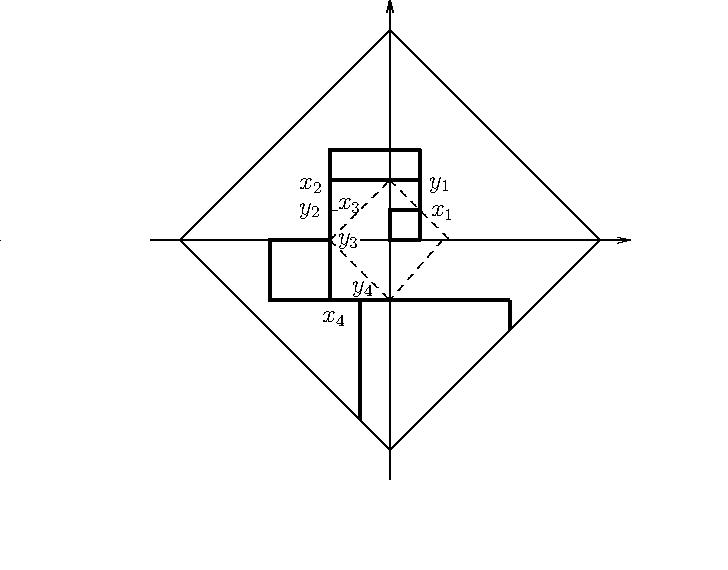
\includegraphics{piv2}
\caption{Os elos pivotais são $e_i=(x_i,y_i)$ para $i=1,2,3,4.$ Note que
$x_3=y_2$ nesta configuração. A linha tracejada é a superfície 
$\del S_{\rho_1}$ de $S_{\rho_1}$. Note os caminhos disjuntos da origem a
$\del S_{\rho_1}$.}
\label{fig:exp2}
\eef
   
No evento $\{\ro_1>r_1\}\cap A_n$, há dois caminhos disjuntos, um de $O$ a  
$\del S_{r_1+1}$ e outro de $O$ a $\del S_n$. Portanto,  
$$\{\ro_1>r_1\}\cap A_n\subset A_{r_1+1}\circ A_n$$  
e a desigualdade de BK produz a desigualdade~(\ref{eq:um}).  
  
Para $k>1$, escreva $$B=\bigcup_{\Ga}\bg,$$  
união disjunta sobre configurações (detalhadas) das salsichas até $y_{k-1}$.  
Então   
\beq  
\p(B,A_n)=\sum_\Ga\p(A_n|\bg)\p(\bg)  
\eeq  
e  
\beq  
\p(\ro_k>r_k,B,A_n)=\sum_\Ga\p(\ro_k>r_k,A_n|\bg)\p(\bg).  
\eeq  
Logo é suficiente mostrar para cada $\Ga$:  
\beq  
\p(\ro_k>r_k,A_n|\bg)\leq\p(A_{r_k+1})\p(A_n|\bg).  
\eeq  
Mas a probabilidade à esquerda é menor ou igual a  
\beqnn 
&\p(\mbox{há caminhos disjuntos abertos de $y_{k-1}$ a 
$\del S(y_{k-1},r_k+1)$ e de $y_{k-1}$}\\ 
&\mbox{}\mbox{a $\del S_n$ que não usam elos dos fechos das salsichas anteriores}), 
\eeqnn 
onde $S(y_{k-1},r_k+1)$ é a esfera de centro em $y_{k-1}$ e raio $r_k+1$.  
  
Como no caso $k=1$, da desigualdade de BK, desta vez aplicada substituindo  
$\ed$ por $\ed\backslash$(elos dos fechos das salsichas anteriores), segue  
que a probabilidade acima é menor ou igual a  
\beqnn  
&\p(y_{k-1}\lr\del S(y_{k-1},r_k+1)\,\,\mbox{sem usar elos anteriores})\\  
&\times\p(y_{k-1}\lr\del S_n\,\,\mbox{sem usar elos anteriores}).  
\eeqnn  
A última probabilidade é igual a $\p(A_n|\bg)$. A primeira é menor ou igual a  
$$\p(y_{k-1}\lr\del S(y_{k-1},r_k+1))$$que, pela invariância translacional do  
modelo, é igual a $\p(A_{r_k+1}).\bo$  
 
\vspace{.5cm} 
A conclusão de que~(\ref{eq:eq4}), e portanto o Teorema~\ref{teo:teo1}, 
segue de~(\ref{eq:eq3}) se dá através do próximo lema, um resultado puramente anal\'\i tico, 
cuja prova será apresentada no apêndice a estas notas. 

\vs

\ble
\label{le:app}
Para $p<\pce$, existe uma constante $\delp$ tal que
\beq
\label{eq:eq6}
\gpn\leq\delp n^{-1/2}.
\eeq
\ele

\vs

\noindent{\bf Prova do Teorema~\ref{teo:teo1}}
De~(\ref{eq:eq6}), temos que
\beq
\label{eq:eq7}
\sum_{i=0}^n\gpi\leq\dep n^{1/2},
\eeq
para algum $\dep$.

Substituindo~(\ref{eq:eq7}) em~(\ref{eq:eq3}), obtemos 
\beq 
\label{eq:eq8} 
\gan\leq\gbn\exp\left[(\b-\a)-c(\b-\a)n^{1/2}\right], 
\eeq 
onde $c$ é uma constante positiva, o que implica~(\ref{eq:eq4}).$\bo$


\vs



É uma conseqüência imediata do Teorema~\ref{teo:teo1} o decaimento exponencial
da função de conectividade.

\vs

\bco
\beq
\label{eq:condec}
\tp(x,y)\leq e^{-\phi_{p}||x-y||_1},
\eeq
com $\phi_{p}>0$ para $p<\pce$.
\eco
(Verifique!)

\vs

Em seguida apresentamos outro corolário ao Teorema~\ref{teo:teo1} 
estabelecendo a suavidade de $\xip$ na fase 
subcr\'\i tica. 
 
\vs

\bco
$\xip$ é $k$ vezes diferenciável em $p<\pce$ para todo $k\geq1$.
\eco

\vs

\noindent{\bf Prova.}

Como $p<\pce$, podemos escrever $\xip$ como
\beq
\xip=\sum_{n=1}^\infty n\p(|C|=n).
\eeq

A última probabilidade pode ser expressa como 
\beq
\label{eq:an1}
\p(|C|=n)=\sum_{m,b}\anb\pem\qb,
\eeq
onde $\anb$ é o número de animais de rede com $n$ sítios, $m$ elos
e $b$ elos de fronteira. Por {\em animal de rede} denotamos conjuntos
conexos de sítios da rede contendo a origem.

Para $n$ fixo, são válidas as seguintes cotas para 
$m$ e $b$ (verifique-as!)
\beq
\label{eq:cotas}
n-1\leq m\leq dn\quad\mbox{e}\quad b\leq 2dn.
\eeq

Estas produzem a seguinte cota para $\sum_{m,b}\anb$
\beqnn
1\geq\sum_{m,b}\anb\pem\qb\ge\sum_{m,b}\anb\pnd\qnd\\
\=(p(1-p)^2)^{dn}\sum_{m,b}\anb,
\eeqnn
do que temos
\beq
\label{eq:kes}
\sum_{m,b}\anb\leq(p(1-p)^2)^{-dn}\leq7^{dn}.
\eeq

Voltando a~(\ref{eq:an1}), temos
\beq
\label{eq:xip}
\xip=\sum_n\sum_{m=n-1}^{dn}\sum_{b=1}^{2dn}n\anb\pem\qb.
\eeq

Vamos dividir o argumento em dois. Para $p=0$,
provaremos o fato mais forte de que $\xip$ é analítica (isto é, pode ser
escrita como série de potências convergente de $p$, o que implica em suavidade).
Em seguida, provaremos suavidade para $0<p<\pce$.

Estendendo $\xip$ formalmente ao plano complexo a partir de~(\ref{eq:xip}), temos
\beq
\label{eq:ser}
\kz=\sum_n\sum_{m=n-1}^{dn}\sum_{b=1}^{2dn}n\anb\zm\zb.
\eeq

Para provarmos analiticidade de $\xip$ na origem, basta mostrarmos 
(pelo Teorema de Vitali), que a série
acima é uniformemente convergente numa região do plano complexo
contendo a origem.

De~(\ref{eq:kes}) temos
\beqnn
\left|\sum_{m=n-1}^{dn}\sum_{b=1}^{2dn}n\anb\zm\zb\right|\le
\sum_{m=n-1}^{dn}\sum_{b=1}^{2dn}n\anb\zam\zab\\
\le n7^{dn}\zan\zad\\
\le A n \czn
\eeqnn
se $|z|\leq1$, onde $A$ depende apenas de $d$ e $c(z)=|z|\{7(1+|z|)^2\}$.

Para $|z|$ suficientemente pequeno, $c(z)<1$ e concluimos que 
a série definindo $\kz$ é uniformemente convergente numa vizinhança
complexa da origem e portanto $\xip$ é analítica em $p=0$.

\vs

Em seguida, vamos diferenciar $\xip$ formalmente $k$ vezes
usando~(\ref{eq:xip}) para obter
\beq
\label{eq:dif}
\difk\xip=\sum_n\sum_{m=n-1}^{dn}\sum_{b=1}^{2dn}n\anb\difk(\pem\qb).
\eeq

Para obter a diferenciabilidade de $\xip$ em $I:=(0,\pce)$, basta mostrar que
a série acima é uniformemente convergente num intervalo fechado arbitrário de
$I$. Para isto notemos que
\beqnn
\left|\difk(\pem\qb)\right|\=\left|\sum_{r=0}^k{k\choose r}
m_rb_{k-r}p^{m-r}(-1)^{k-r}(1-p)^{b-(k-r)}\right|\\
%
\le\pem\qb\sum_{r=0}^k{k\choose r}(m/p)^r(b/(1-p))^{k-r}\\
%
\=\pem\qb\left(\frac{m}{p}+\frac{b}{1-p}\right)^k,
\eeqnn
onde $x_r=x!/r!$. Logo,
\beqnn
&&\sum_{n\geq
N}\left|\sum_{m=n-1}^{dn}\sum_{b=1}^{2dn}n\anb\difk(\pem\qb)\right|\\
%
\le\left(\frac{2d}{p(1-p)}\right)^k\sum_{n\geq N}n^k
\sum_{m=n-1}^{dn}\sum_{b=1}^{2dn}n\anb\pem\qb\\
%
\=\left(\frac{2d}{p(1-p)}\right)^k\sum_{n\geq N}n^k\p(|C|=n)
\eeqnn
e, portanto, (\ref{eq:exp1}) implica na convergência uniforme de~(\ref{eq:dif}) em
intervalos fechados de $I$. $\bo$

\vs

\bob
Um argumento semelhante ao da prova acima, mas usando o decaimento {\em
exponencial} da distribuição de $|C|$ (como discutido na
Observação~\ref{ob:exp1}), prova analiticidade de $\xip$ em $(0,\pce)$.
(Vide~\cite{kn:G}.)
\eob

























 
 
 

